\documentclass{article}
\usepackage{tikz}
\usetikzlibrary{shapes.geometric, arrows, positioning, calc}
\usepackage{geometry}
\usepackage{amsmath}

\begin{document}

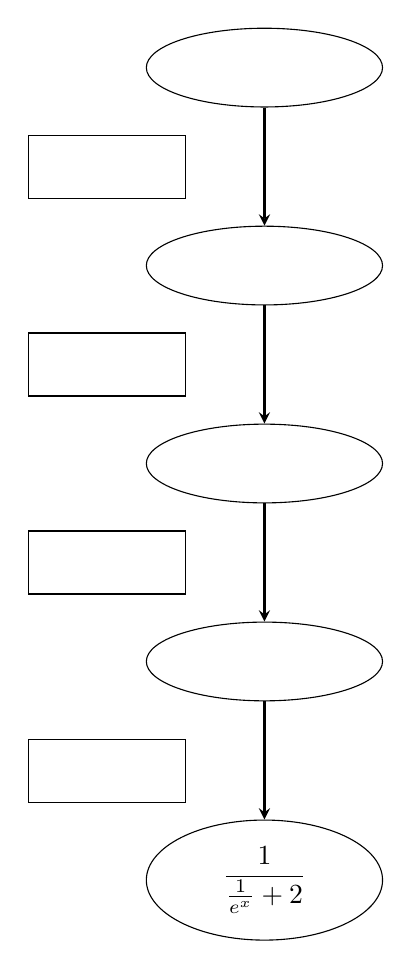
\begin{tikzpicture}[node distance=1.5cm and 1cm]

% Definir estilos para nodos
\tikzstyle{oval} = [ellipse, draw, minimum width=3cm, minimum height=1cm, align=center]
\tikzstyle{rect} = [rectangle, draw, minimum width=2cm, minimum height=0.8cm, align=center]
\tikzstyle{arrow} = [->, >=stealth, thick]

% Nodos verticales (funciones)
\node[oval] (f1) {};
\node[oval] (f2) [below=of f1] {};
\node[oval] (f3) [below=of f2] {};
\node[oval] (f4) [below=of f3] {};
\node[oval] (f5) [below=of f4] {$\dfrac{1}{\frac{1}{e^x} + 2}$};

% Rectángulos a la izquierda
\node[rect] (l1) at ($(f1)!0.5!(f2) + (-2,0)$) {};
\node[rect] (l2) at ($(f2)!0.5!(f3) + (-2,0)$) {};
\node[rect] (l3) at ($(f3)!0.5!(f4) + (-2,0)$) {};
\node[rect] (l4) at ($(f4)!0.5!(f5) + (-2,0)$) {};
%\node[rect] (l5) {};

% Flechas entre funciones
\draw[arrow] (f1) -- (f2);
\draw[arrow] (f2) -- (f3);
\draw[arrow] (f3) -- (f4);
\draw[arrow] (f4) -- (f5);

\end{tikzpicture}

\end{document}